% !TEX encoding = UTF-8
% !TEX program = pdflatex
% !TeX spellcheck = en_GB
% !BIB = biber

\documentclass[english]{article}
\usepackage{amsmath}
\usepackage{wasysym}
\usepackage{amssymb}
\usepackage{subcaption}
\usepackage{tabularx}
\usepackage{babel}
\usepackage[utf8]{inputenc}
\usepackage{graphicx}
\usepackage[obeyspaces]{url}

\usepackage{titlesec}

\setcounter{secnumdepth}{4}
%%per paragrafi -----
\titleclass{\subsubsubsection}{straight}[\subsection]

\newcounter{subsubsubsection}[subsubsection]
\renewcommand\thesubsubsubsection{\thesubsubsection.\arabic{subsubsubsection}}
\renewcommand\theparagraph{\thesubsubsubsection.\arabic{paragraph}} % optional; useful if paragraphs are to be numbered

\titleformat{\subsubsubsection}
  {\normalfont\normalsize\bfseries}{\thesubsubsubsection}{1em}{}
\titlespacing*{\subsubsubsection}
{0pt}{3.25ex plus 1ex minus .2ex}{1.5ex plus .2ex}

\makeatletter
\renewcommand\paragraph{\@startsection{paragraph}{5}{\z@}%
  {3.25ex \@plus1ex \@minus.2ex}%
  {-1em}%
  {\normalfont\normalsize\bfseries}}
\renewcommand\subparagraph{\@startsection{subparagraph}{6}{\parindent}%
  {3.25ex \@plus1ex \@minus .2ex}%
  {-1em}%
  {\normalfont\normalsize\bfseries}}
\def\toclevel@subsubsubsection{4}
\def\toclevel@paragraph{5}
\def\toclevel@paragraph{6}
\def\l@subsubsubsection{\@dottedtocline{4}{7em}{4em}}
\def\l@paragraph{\@dottedtocline{5}{10em}{5em}}
\def\l@subparagraph{\@dottedtocline{6}{14em}{6em}}
\makeatother

\setcounter{secnumdepth}{4}
\setcounter{tocdepth}{4}
%% --------
\graphicspath{{./images/}}
\usepackage{hyperref}
\hypersetup{
    colorlinks=true, 
	linkcolor=blue, 
	filecolor=blue, 
	citecolor = black,       
	urlcolor=blue, 
}
\usepackage{listings}
\lstset{
  xleftmargin=15pt,
  xrightmargin=0pt,
  framexleftmargin=0pt,
  framexrightmargin=0pt,
  basicstyle={\fontsize{9pt}{10pt}\ttfamily},
  columns=flexible,
  numbers=left,
  numbersep=10pt,
  numberstyle={\fontsize{9pt}{11pt}\selectfont\color[rgb]{0.4,0.4,0.1}},
  keepspaces=true,
  showstringspaces=false,
  identifierstyle=\color[rgb]{0.1,0.1,0.1},
  keywordstyle=\color{blue},
  commentstyle=\color[rgb]{0,0.3,0},
  morekeywords={rule, lemma},
  morekeywords=[2]{let, in},
  morekeywords=[3]{Fr, pk},
  morekeywords=[4]{In, Out},
  morekeywords=[5]{senc, aenc, h}
  morecomment=[s][keywordstyle3]{/*}{/},
  keywordstyle=\color[rgb]{0.44,0.57,0.65},
  stringstyle=\color{green},
  keywordstyle=[2]{\color[rgb]{0.86,0.57,0.18}},
  keywordstyle=[3]{\bfseries\color[rgb]{0,0.3,0.2}}
  }
\usepackage{biblatex}
\addbibresource{thud.bib}

\title{An overview and analysis of Apple’s AirTag technology and FindMy service}
\author{Zanolin Lorenzo}
\date{February, 2024}
\begin{document}

\maketitle

\tableofcontents
\newpage

% scaletta:
%% history
%% Airtag section
%%  UWB
%%  Bluetooth
%%  Sw
%% Security
%% Applications and mods

\begin{abstract}
  The main goal of this project is to dig into how Apple AirTags work, including their setup, security measures, and uses; since everything is tied to the FindMy network and the UWB technology, we will also look into the security methods used in this network and the basic principle of the Ultra-Wideband (UWB). The idea is to get a clear picture of how Apple AirTags are put together, how secure they are, and the different ways they're used in the FindMy network.
\end{abstract}

\section{Introduction}\label{sec:intro}
In the rapidly evolving landscape of technological advancements, Apple's AirTags have emerged as an innovation, offering a solution to tracking and locating personal belongings. This paper delves into the architecture and security of AirTags, with a particular emphasis on the UWB technology that underlies their functionality. Moreover, as AirTags operate within the framework of the FindMy network, this exploration extends to an overview of the security measures embedded in both the device and the overarching network; through the examination of the relationship between AirTags, UWB, and FindMy security, this paper seeks to provide insights of the working principles of the ecosystem which enables accurate location tracking, while also addressing concerns related to privacy and data security. 

%DA RIFARE We will go over the fundamentals of UWB technology in Section \ref{sec:uwb} and examine its benefits from a security standpoint. In Section \ref{sec:find}, we will delve deeper into the examination of the FindMy network. We will begin with providing a general overview of the architecture, go on to a functioning example and end with a security analysis of the whole thing. Lastly, we will conduct a thorough examination of the AirTag concept in Chapter \ref{sec:at}, concentrating on the architecture (first examining the software component, then the hardware component) and then moving on to the security analysis of this technology.

\section{AirTag}\label{sec:at}
An AirTag is a small device from Apple which is intended to assist users in finding and monitoring objects that are easily misplaced or lost, such as wallets, bags, and keys.
\subsection{Overview}
 By connecting to compatible Apple devices (iPhones, iPads, and Macs) through Bluetooth, the AirTag enables users to locate the linked object and, subsequently, the AirTag itself using the Find My app. In order to help with lost item recovery, the gadget has capabilities including accurate location tracking, proximity notifications and a Lost Mode. Its design prioritizes privacy and security, safeguarding user data through the use of encryption and anonymization. With the introduction of iOS 14.5 and iPadOS, Apple has introced the support for AirTags.
\subsection{History}
\subsection{Architecture}
First of all, this devices utilize two technologies: UWB and Bluetooth; we will briefly look at both of them.
\subsubsection{UWB}\label{sec:uwb}
\subsubsubsection{Overview}
Within the domain of wireless communication technologies, UWB operates by employing extremely low-power, short-duration pulses that span a broad spectrum and result in increased distance measuring precision, allowing for high data transfer rates and precise positioning capabilities over a wide frequency range, typically several gigahertz. Originally conceived for military and radar applications, it has gradually invaded diverse sectors, finding particular prominence in consumer electronics, healthcare, automotive systems, and the Internet of Things (IoT).

From \cite{Coppens2022}: ``UWB achieves real-time accuracy because the receiver can determine the time of arrival of the signal, allowing centimeter-level accurate ranging using techniques such as Time-of-Flight (ToF)\footnote{From \cite{tof}, ``Time of flight is the measurement of time taken to travel a distance in order to determine distance, speed, or properties of the medium".}, Time Difference of Arrival (TDoA)\footnote{From \cite{tdoa}, ``TDoA is a positioning methodology that determines the difference between the time-of-arrival (ToA) of radio signals. TDoA is used in a real-time location system (RTLS) to accurately calculate the location"} and Two-Way Ranging (TWR)\footnote{From \cite{twr}, ``The Two Way Ranging method determines the Time of Flight of the UWB RF signal and then calculates the distance between the nodes by multiplying the time by the speed of light."}. Combining with error correction techniques, the ranging error can be as low as 58 mm".

Because of its wide spectrum utilization, UWB can coexist peacefully with other wireless technologies and send out massive volumes of data quickly; also, it has a reduced range of operation due to the wide radio bandwidth it uses (according to \cite{Zafar2019}, ``U1 chip can emit data using two frequencies: 6.24 GHz and 8.2368 GHz. The FCC has allocated ultrawideband a spectrum starting from 3.1GHz to 10.6GHz."). To overcome this problem, we can use an antenna of type \textit{MIMO} (multiple-input and multiple-output) to enhance UWB's range; this kind of devices can be embedded into our everyday devices due to their reduced size. From \cite{di2006uwb}: ``due to the low energy density and the pseudo-random (PR) characteristics of the transmitted signal, the UWB signal is noise-like which makes unintended detection difficult".

According to \cite{aps}, ``Apple-designed U1 chip uses UWB technology for spatial awareness, allowing iPhone 11, iPhone 11 Pro and iPhone 11 Pro Max or later iPhone models to precisely locate other U1-equipped Apple devices"; this means that when two U1 devices come close to each other, the two start measuring their exact distance using ToF. According to IEEE 802.15.4a \cite{5394030}, ``UWB can determine the relative position of other devices in the line of sight even up to 200 meters", which means that we can leverage this technology to track items that are very close to us and those that are relatively distant.

It is important to distinguish the differences between Bluetooth Low Energy (BLE) and UWB. The former allows for detecting a device but cannot accurately measure its position, as it relies on the device's range. UWB, on the other hand, enables precise localization of the device by measuring the position based on the time interval between when the signal leaves point A and when it arrives at point B.
Table \ref{tableu} represents the principal differences between the two technologies, data is taken from \cite{encstore}:
\begin{table}[h] 
\caption{BLE-UWB comparison.}
  \centering
  
    \begin{tabular}{l|l|l|}
      \cline{2-3}
      {}                               & {\textbf{UWB}}                & { \textbf{Bluetooth (BLE Beacons)}} \\ \hline
      \multicolumn{1}{|l|}{{  \textbf{Battery}}}  & {  Low consumption}             & {  Low consumption}                  \\ \hline
      \multicolumn{1}{|l|}{{  \textbf{Data Rate}}}  & { 1 Gbps }             & { 2 Mbps }                  \\ \hline
      \multicolumn{1}{|l|}{{  \textbf{Range}}}    & {  up to 200 meters} & {  up to 100 meters}       \\ \hline
      \multicolumn{1}{|l|}{{  \textbf{Accuracy}}} & {  10 centimeters} & {  up to a meter}                    \\ \hline
      \multicolumn{1}{|l|}{{  \textbf{Cost}}}     & {  Low}                         & {Depend on the context }                              \\ \hline
    \end{tabular}
    \label{tableu}
  \end{table}

\subsubsubsection{Security analysis}
The fact that UWB pulses are resistant to the multipath effect\footnote{From \cite{Figueroa2022}: ``Multipath interference occurs when a signal from a transmitter arrives at a receiver via two or more routes; typically there is a direct path plus a number of indirect paths caused by reflections".} is one of its key characteristics. This occurs when radio waves are reflected or refracted by artificial or natural objects near the primary signal channel, causing the signal to reach the receiver via many paths. Positioning accuracy is improved by immunity to the multipath effect, particularly when compared to other technologies that are more vulnerable. Moreover, UWB's resilience to jamming and narrowband fading makes it a particularly reliable technology choice, even when several UWB systems are being used at once.

Another important aspect to consider is the resistance to Relay Attacks, which is a vulnerability of the majority of signal-based architectures; we will present a concrete example taken from \cite{Global_2020}. In this attack, the goal is to trick a car into thinking the key and owner are close by using two people with hacking devices. The first relays signals from the car to the second thief, who transmits the signal to the house. The key responds, allowing entry into the car. The relay attack intercepts and amplifies wireless signals used to unlock the door and start the car, despite the key's distance. With UWB, that would not be possible due to its working scheme: to ensure the car doesn't have to make assumptions, rapid measurements are utilized to establish distance very precisely. Any attempt to relay attack or intercept the UWB signal will merely cause the answering device's acknowledgement signals to arrive later, indicating to the car that the real key is actually farther away. The car's presumption is replaced with assurance when using UWB, which greatly increases the security of the passive keyless entry system.

The implemented security measures, taken by Apple, are the following: MAC address randomization and frame sequence number randomization \cite{aps}.

\paragraph{MAC address randomization}
From \cite{aps}: ``Apple platforms use a randomized media access control address (MAC address) when performing scans when not associated with another device. Because a device’s MAC address changes when disconnected from another device, it can’t be used to persistently track a device by passive observers of traffic". This provides us with a level of protection against visibility from malicious individuals attempting to sniff the traffic for malicious purposes.

\paragraph{Frame sequence number randomization}
From \cite{aps}: ``Apple devices randomize the sequence numbers whenever a MAC address is changed to a new randomized address". As before, this addition increases the privacy, also avoid the possibility of replay attacks.


\subsubsection{Bluetooth}
%.... da fare


Now, we will analyze the architecture of this product; the information has been reverse engineered by Adam Catley in \cite{reverse}. We will cover both the hardware and software aspects of this kind of device.
\subsection{Software analysis}\label{sec:beacons}
As for the software part, we will present informations taken from \cite{reverse}: ``there are various states in which AirTag can be; we will now quickly present all of them.
\begin{itemize}
  \item \textit{Not registered}: when removed from FindMy network or reset, the AirTag is brand new and every 33 milliseconds, it advertises itself as it waits to be connected.
  \item \textit{Initialisation}: a public/private key pair is created and shared by the AirTag and the linked iOS device after it is registered to an Apple ID.
  \item \textit{Connected}: the owner’s device is in range. No broadcasts occur.
  \item \textit{Disconnected}: the owner’s device is out of range. Broadcasts identity every 2000 ms.
  \item \textit{Out of sync}: happens when an AirTag reboots while separated from its owner’s device. Acts like Disconnected but absolute time is lost, so events are relative to time since power-up. Identity resets to its initial value.
  \item \textit{Lost}: occurs 3 days after Disconnected or Out of sync begins. Moves to Waiting for motion every 6 hours.
  \item \textit{Waiting for motion}: samples the accelerometer every 10 seconds until motion is detected.
  \item \textit{Sound alert}: a command to play a noise is received from either a connected device or by detecting motion. Lasts a maximum of 20 seconds.
  \item \textit{Precision finding}: triggered by the owner’s device while Connected. Is overridden by Sound alert."
\end{itemize}
As we will see in Section \ref{hw}, even if the finder has an Android device, they may be able to identify the owner of an AirTag thanks to its NFC antenna. Depending on its current status, the tag carries a URL that uniquely identifies the AirTag. It can only be read when the AirTag is turned on (meaning that the battery within it is sufficiently charged). There are some parameters that are attached to the URL, used to identify the device; we will briefly present them. These informations were presented in \cite{reverse}, ``Keep in mind that all of the following parameters are fixed for a single unit, even after power cycles, long runtime, resets and modes.
\begin{itemize}
  \item \textit{pid}: product ID for AirTag.
  \item \textit{b}: something related to the battery.
  \item \textit{pt}: UWB Precision Tracking version.
  \item \textit{fv}: firmware version.
  \item \textit{dg}: something related to diagnostic.
  \item \textit{z}: unknown.
  \item \textit{bt}: Bluetooth address; will be present only when Unregistered.
  \item \textit{st}: serial number of the tag (the one printed on the device under the battery); will be present only when Unregistered.
  \item \textit{bp}: Bluetooth protocol version; will be present only when Unregistered."
\end{itemize}
In the \textbf{Unregistered} state, the stored URL has the following format:
\url{https://found.apple.com/airtag?pid=5500&b=00&pt=004c&fv=00100e10&dg=00&z=00&bt=A0B1C2D3E4F5&sr=ABCDEF123456&bp=0015}

According to \cite{reverse},
``Once the device is \textbf{registered}, the parameters \textit{bt, sr, bp} will be removed and replaced with a single anonymous identifier \textit{pi}, which is the only parameter that changes at least every 15 minutes when the Bluetooth address and/or the advertising data changes". Probably, it is the P-224  $p_i$ presented in \ref{keys} or the SHA-224 of it. 


The device operates on a schedule designed to optimize its functionality:
at 4:00 am every day, it updates its BLE address and public key, ensuring secure communication channels.
Advertisement data is refreshed every 15 minutes, guaranteeing that nearby devices receive the most current information.
Should it become separated from its owner's device for three days, the device enters a lost mode, activating specific features to aid in recovery efforts.
While in this lost mode and detecting movement, the device emits a noise every 6 hours to alert nearby individuals.
To conserve energy while remaining responsive, the accelerometer is sampled every 10 seconds while waiting for motion; upon detecting movement, its sampling frequency increases to every 0.5 seconds for 20 seconds, providing detailed tracking data.
When it's away from the owner, the device transmits BLE advertisement signals every 2 seconds enhancing its detectability.
Finally, in close proximity to its proprietor's device, the tag establishes a BLE connection interval of 1 second, ensuring efficient communication and responsiveness.
\subsection{Hardware analysis}\label{hw}
As for the hardware part, an important aspect comes to light: all of the used components, aside the Apple's U1 UWB chip, are off the shelf, as we can see in Figure \ref{img:pcb}.
Each AirTag has three antennas: one for BLE that works at 2.4 GHz, one for NFC at 13.56 MHz and finally the UWB one at 6.5-8 GHz.
We have a plastic case that works as a diaphragm and it is adhered to the voice coil. When the coil is energized, the fixed magnet causes it to move back and forth, creating sound and serving as the speaker.
If motion is detected, the speaker will loudly beep for up to 20 seconds after being away from its owner for three days. After that, it will be silent for the following six hours before watching for movement once more.
\begin{figure}[ht]
	\centering
	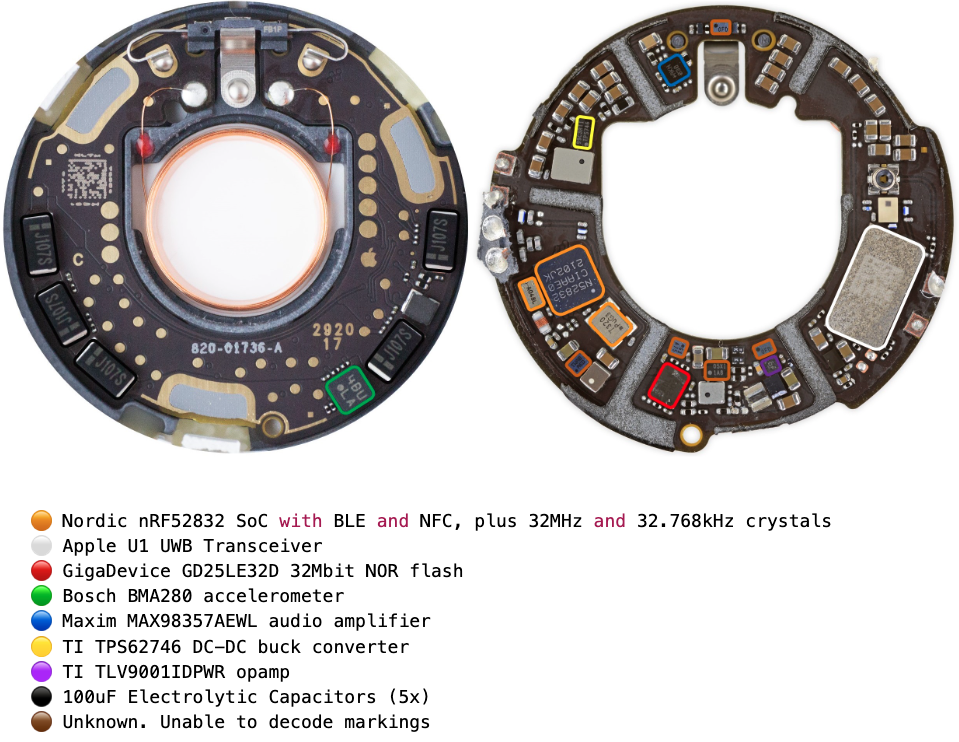
\includegraphics[width=\textwidth]{images/pcb.png}
	\caption{PCB overview (image from \cite{reverse}). }
	\label{img:pcb}
\end{figure}

\subsection{Security Analysis}\label{sec}
Security-wise, from \cite{reverse} it has emerged that no security checks are performed on the device during its operation; in fact, none of the data in the AirTag is protected from tampering or disclosure.
\subsubsection{Vulnerabilities}\label{sec:vuln}
We will present some vulnerabilities that have been found by by Adam Catley in \cite{reverse}; Table \ref{vuln} resumes them.
\paragraph{Exploitable voltage levels}
The Nordic nRF52832 has the function Access Port Protection \cite{nordicsemi} that it is used to prevent external parties from reading the internal memory and to limit access to the Debug Port via SWD\footnote{From \cite{Oberli_2019}, ``SWD is a standard for debugging and accessing microprocessor registers. This protocol has been in use for many years and is still in use today."}; however, according to \cite{side}, side channel attacks are effective against this mechanism, more specifically voltage glitching. Consequentially, ``it is possible to extract Bluetooth pairing keys to connect to the owner’s phone or run (on the AirTag) a custom firmware since Apple does not check the signature of it (the firmware)", from \cite{reverse}. In this case, if an attacker is able to use voltage glitching to inject a modified firmware, maybe he can use it to track the owner and it will not be discovered since the anti-stalking countermeasures presented in \ref{countermeasures} do not work with personal objects. According to \cite{voltage}, ``the only way to guarantee the security of the voltage glitch detection circuitry protecting an SoC or microcontroller is to implement the detector on the chip itself. An example of detector is Voltage Glitch Detector IP from INVIA, which provides comprehensive protection against power glitching attack. It detects positive and negative supply voltage glitches, and has a slope detection range between 100 MV/s and 2 GV/s".

\paragraph{Insecure Storage}All the informations saved into the GD25LE32D 32Mbit NOR flash are in clear, as we can see in \cite{tweet}; also, the nRF52832 does not have any encrypting functionality. In this case, we don't know if this is a real vulnerability since we do not know whether the FindMy private key-pair is stored inside the AirTag. However, an attacker can read without problems all the information that is stored within the device and, in general, this behavior can be exploited (maybe in the future) to inject malicious data into the AirTag or to read sensible informations. To prevent this, we can implement encryption via software or hardware; typically, on small devices, it is better to use dedicated hardware circuitry to encrypt data.

\paragraph{Unathenticated transmission}The only way to identify an AirTag is to use its public key, which is transmitted via BLE advertising packets; this identification does not require authentication. These IDs can be recorded and replayed by any nearby BLE device to mimic the appearance of the real AirTag. Let's see an example taken from \cite{reverse}: ``an attacker steals a personal item containing an AirTag and subsequently records the current public identity before removing the battery. At this point, the identity can be relayed to any BLE device in a decoy location to give the owner a false search area to recover their property". In this case, the AirTag is exploited to steal personal belongings from the owner. To avoid this, Apple can use authenticated encryption; for example, we can use GCM, which offers the ability to verify the authenticity and integrity of extra authenticated data (AAD) that is provided in clear text in addition to authenticated encryption (confidentiality and authentication). More details can be found in \cite{gcm}.

\begin{table}[h] 
  \caption{Vulnerabilities.}
  \centering
  \begin{tabularx}{\textwidth}{|X|X|X|}
    \hline
    \textbf{Vulnerability}      & \textbf{Possible attack} & \textbf{Countermeasure}             \\ \hline
    Exploitable voltage levels  & Side-channel attack      & Use detector         \\ \hline
    Insecure storage            & Memory-reading attack    & Implement hardware encryption \\ \hline
    Unauthenticated transmission & Replay attack            & Implement authenticated encryption                     \\ \hline
  \end{tabularx}
  \label{vuln}
\end{table}

\subsubsection{Anti-stalking countermeasures}\label{countermeasures}
An important aspect that has emerged with the AirTags is the stalking problem. Stalking using AirTags refers to the potential misuse of Apple's AirTag tracking devices to monitor and track individuals without their consent; these small devices are designed to help users locate misplaced items. However, due to their small size and long battery life, AirTags could potentially be used for nefarious purposes, such as stalking. An individual could secretly place an AirTag on someone's belongings and then use the Find My app to monitor their movements in real-time. Since AirTags are designed to be difficult to detect, the victim may not realize they are being tracked for an extended period of time.

Apple has implemented measures to prevent the misuse of AirTags, including alerts and notifications for when an unknown AirTag is detected near a user's device, as well as features like Precision Finding, which can help users locate unwanted AirTags. The first line of defense in the event that someone plants an AirTag on a victim's belongings might be an alert to his iPhone indicating the presence of a foreign AirTag. Apple built the iPhone-AirTag connection to do this in two ways: either when you get to the place that your iPhone's machine learning intelligence has detected as home (or when you manually record it as home) or after the AirTag has stuck with you for a certain ``continuous" period of time that Apple deems sufficient to be considered abnormal. This seems perfect; however, if the victim has a non Apple device, such as an Android phone this could be a problem. To prevent this problem, Google and Apple collaborated to develop Unknow Tracker Alerts, which is a feature that was announced during the Google I/O 2023 opening presentation.

An important factor is that AirTags can emit sounds when they are separated from the owner's devices for an extended period of time. This way, a victim of a stalking attempt can hear the noise emitted by the device and realize they are being tracked. More precisely, three days following separation is when sound alerts begin; even in that case, Once the tag detects movement, it will emit a sound for about 20 seconds, followed by at least 6 hours of silence (even if further movements are detected). As correctly observed by Catley in \cite{reverse}, ``the problem with this is that three days can be enough to study the victim's routine and after that period, it is likely to make noise for a maximum of 40 seconds a day during a normal commuting schedule. Movement is likely to coincide with a noisy environment while traveling or be muffled by objects touching the white casing, meaning that the victim won't realize it". According to \cite{server}, ``the frequency and duration of sounds can be adjusted from the Apple server side", meaning that Apple can increase both of them to avoid situations in which the victim is unable to hear the sounds.

However, despite these safeguards, the potential for AirTags to be used for stalking remains a concern; in fact, a problem is that the voice coil can be disconnected without disassembly. The resulting problem is that an AirTag can function normally without the voice coil, and therefore, if used for stalking, it will be difficult for a user without an Apple device to detect its presence if it is well hidden.

\section{FindMy network}\label{sec:find}
\subsection{Overview}
Apple created the technology, known as the FindMy network, which is intended to assist consumers in finding their compatible third-party accessories, such as Apple AirTags, as well as their Apple devices, including iPhones, iPads, Macs, and AirPods. By utilizing UWB and BLE technologies, the FindMy network facilitates accurate and instantaneous location tracking.

Apple merged the applications Find My Friends and Find My iPhone together into a single one called \textit{Find My}, allowing users to locate everything they need in one place. Subsequently, Apple has consistently enhanced the Find My app, incorporating functionalities such as monitoring when a iPhone is disconnected, when it is turned off and when it has been wiped.

You can access the sections of the app by touching the tabs located at the bottom. \textit{People} are located on the left and represents your friends location (they have to share it with you in order to be visible), while your personal belongings, including Bluetooth goods with Find My functionality and AirTags, are located in the center; finally, on the right, there's a \textit{Me} tab with all of your settings and info, as we can see in Figure \ref{findmy2}.

There are several useful features within this app, we will present some examples taken from \cite{Clover_2022}:
\begin{itemize}
  \item \textit{Separation alerts}: you will get notified if you unintentionally leave behind an Apple device, an AirTag-tagged item or a third-party device that has enabled Find My features.
  \item \textit{Locating friends and sharing location}: this feature allows you to share your location with friends or family so they can view it when needed. One useful aspect of this function is that it also enables you to monitor your children or individuals with certain orientation problems, helping them if they get lost.
  \item \textit{Locating devices without connection}: this feature is very useful as it allows offline devices to be tracked using the FindMy network. Essentially, a lost device uses BLE to send beacon packets to nearby Apple devices, which then send the encrypted location to the owner's iCloud account. As we will see later, it will also be possible for some devices to be located even without battery charge, meaning when the device is turned off.
  % ovviamente se il bluetooth è off allora non è rilevabile, non basta avere il chip U1 alimentato
  \item \textit{Anti-stalking measures}: this feature helps prevent situations where a malicious individual secretly places a device belonging to a FindMy network in your belongings to track your location in real time, using your device to upload its position. When your device receives multiple BLE beacons from a nearby device, it will notify you that you might be tracked by a device and ask if you want to disable its location sharing. We will also come back on this following the studies done in \cite{airguard}.
  \item \textit{Precision finding}: this feature requires the presence of the U1 chip, which uses UWB technology to locate another device equipped with the same chip. It is very useful for precisely locating AirTags, which are often attached to items that we tend to lose frequently. The range of this technology is limited to that of UWB, as we previously discussed.
\end{itemize}

\begin{figure}[t]
	\centering
	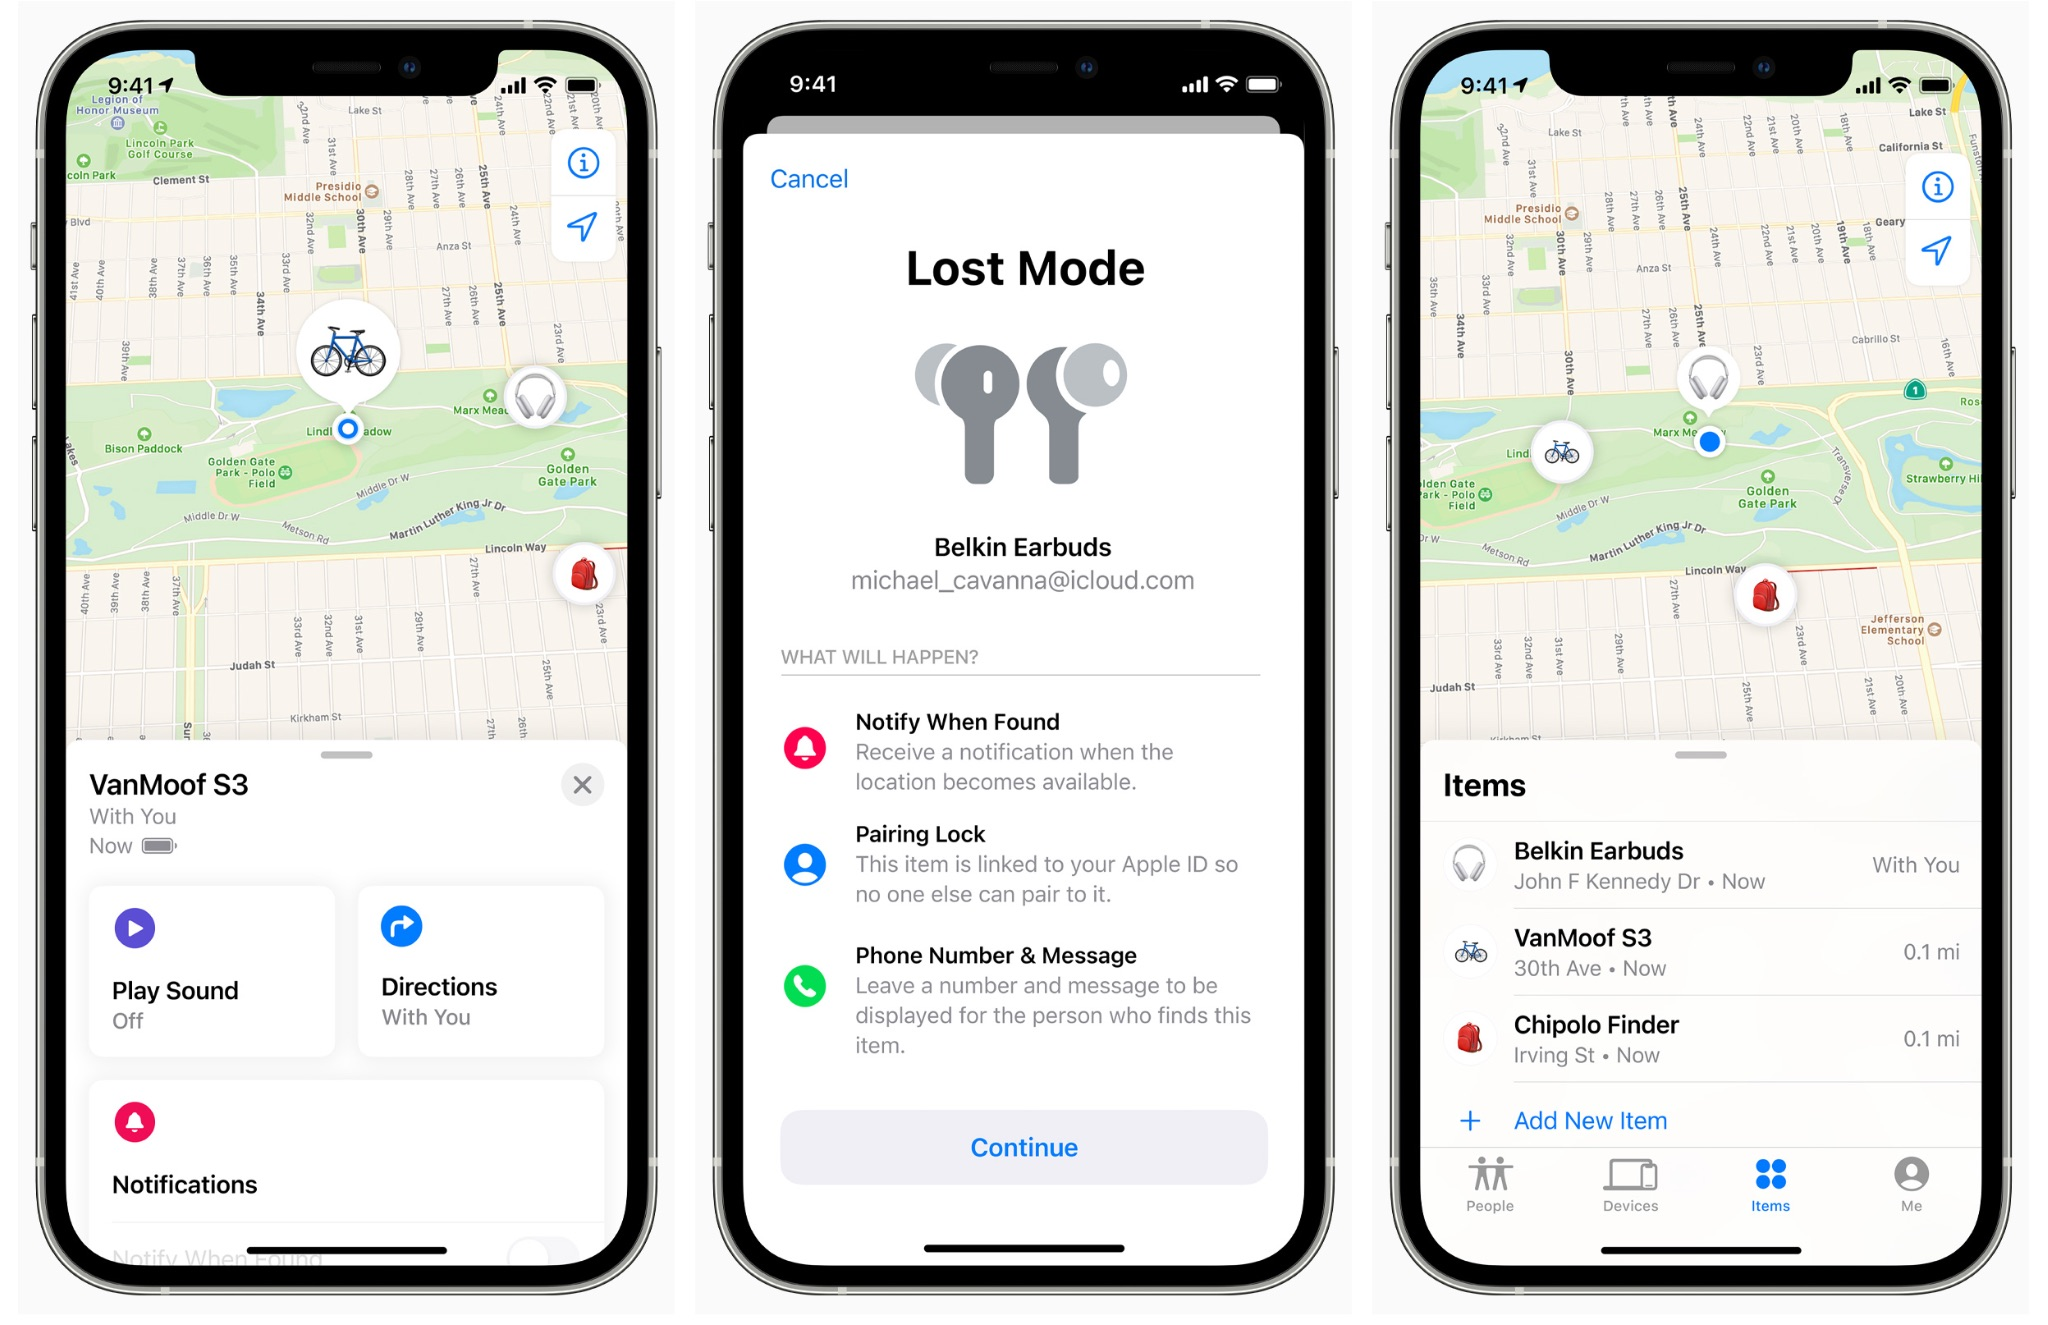
\includegraphics[width=.9\textwidth]{images/findmy.jpg}
	\caption{FindMy screenshots (images from \cite{findmyscreen}).}
	\label{findmy2}
\end{figure}

\subsection{Functioning}
%As for the functioning, we will use the content of \cite{Mayo_2021,Itani_2021,Clover_2022,OBoyle_2021} to describe the entire process. 
Now, we will describe the entire functioning process. First of all, we want to register our products within the application; in the case of a non-accessory item, it will automatically be inserted in the \textit{Devices} section. In the case of accessories, like AirTag, you need to manually add them using the \textit{Items} section.

Now you should be able to localize online devices from the map; in the case of a close AirTag you can also use the \textit{Precision finding} to locate the object using U1 chip, as represented in Figure \ref{findmy1}. As always, Apple creates an excellent graphical interface for its features; for instance, Precision Finding utilizes multiple components. From \cite{OBoyle_2021}: ``the technology fuses input from the iPhone's camera, ARKit, accelerometer and gyroscope in order to guide the user to their AirTag using a combination of sound, haptics, and visual feedback." 

\begin{figure}[t]
	\centering
	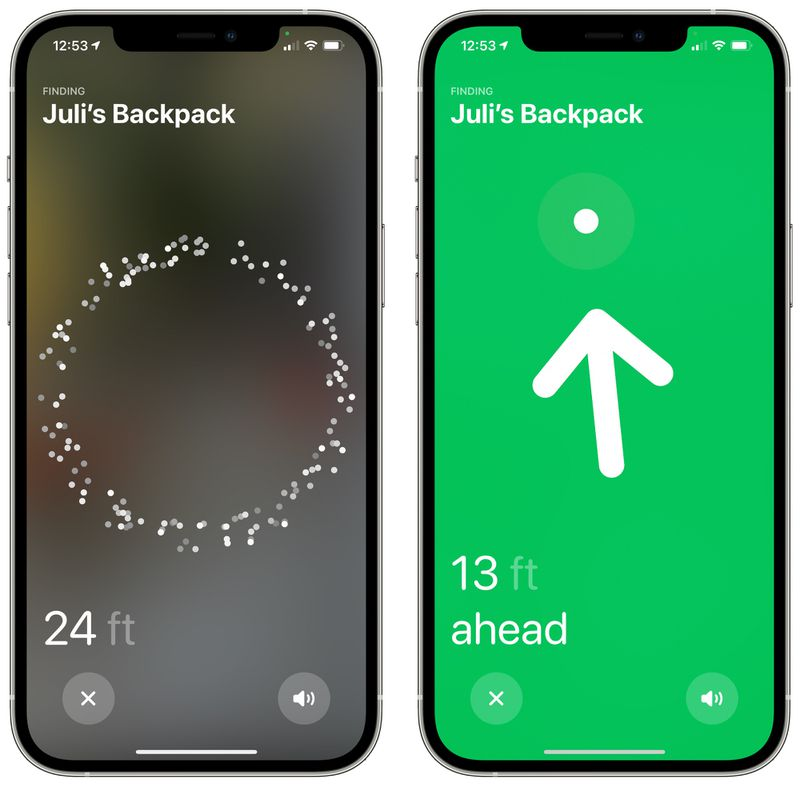
\includegraphics[width=.6\textwidth]{images/airtag-precision-finding-2.jpg}
	\caption{Precision Finding.}
	\label{findmy1}
\end{figure}

In case of a stolen device, you can always activate \textit{Lost Mode}; it will send you a notification as soon as the iphone is detected, which means that if the phone is connected to a network or via BLE to other Apple devices, the owner will receive a message from FindMy containing the position of the device. Also, in this modality, all the registered cards in Apple Pay will be temporarily disabled.

This technology seems pretty useful already, but if a device is powered off, how can it be localized? If you device is U1-equipped, its Bluetooth is enabled and its iOS version is at least 15 then it can be localized even if turned off. From \cite{Mayo_2021}: ``with iOS 15, your iPhone is still traceable through the Find My network even when the device is powered off. 
It seems that with iOS 15, the phone is not really fully powered off, it stays in a low-power state and acts like an AirTag, allowing any nearby iOS device to pick up the Bluetooth signal and send back its location.
This also means if the iPhone runs out of battery during the day, the owner still has a chance of finding its location for several more hours. As long as Activation Lock is activated and the phone is restored to factory settings, Apple claims that location tracking will continue to function". This seems very useful for iPhones, but what about other devices, like Macbooks? Since Apple has not commented on the matter, the author conducted some tests and discovered that even machines with high specifications lack the U1 chip and are therefore not localizable when turned off. 

Like other devices registered on FindMy, AirTags can also be located by other Apple devices in the same manner as written before. Specifically, as we will see in the Section \ref{sec:beacons}, once an AirTag moves out of proximity range of the owner's other devices, it begins to send BLE beacons to be identified and detected on FindMy. The only way to stop an AirTag from being fully detectable is to remove the CR2032 coin battery (or when it fully discharges).

\subsection{Security analysis}
In this section, we will analyze the security measures implemented in FindMy to increase the safety of the architecture. Let us add some more details to the process of localizing an object.
\subsubsection{Preliminars definitions}
We will first define a few terms taken from \cite{whocanfind}:
\begin{itemize}
  \item \textit{Owner Devices}: Apple devices owned by the user that can be located; the complete list of detectable devices is available in \cite{Apple}. Within the FindMy section of your iCloud account, you can view the location of all your devices.
  \item \textit{Lost Devices}: There are two types of devices that can be considered lost; according to \cite{whocanfind}, ``Apple devices are classified as lost when they lose internet connectivity. Third-party accessories \cite{gadget} are compact, battery-powered devices that can be affixed to personal items and are configured via the owner's device. Accessories are considered lost when they lose their BLE connection to the owner's device"; as we will see in section \ref{sec:crypto}, these devices start sending BLE beacons to be detectable by other Apple devices.
  \item \textit{Finder Devices}: Apple devices that are capable of localizing lost devices. According to \cite{whocanfind}, ``the only iPhones and iPads with a GPS module will be able to use a finder. By looking for BLE ads, finder devices can identify misplaced gadgets and accessories. A finder device sends an end-to-end encrypted location report, including its current location, to Apple's servers after intercepting an advertisement. We will see what the contents of the report are".
  \item \textit{Apple’s Servers}: They are used to store all location reports sent by the various finder devices, and only the respective parties can access and download them locally. All information is encrypted, and only those with the private key can access it, namely the owners of the involved devices.
\end{itemize}
\subsubsection{Workflow}
From \cite{aps}, page 202: ``An online device can report its location to the user via iCloud. Find My works offline by sending out short range BLE signals from the missing device that can be detected by other Apple devices in use nearby. Those nearby devices then relay the detected location of the missing device to iCloud so users can locate it in the Find My app while protecting the privacy and security of all the users involved". An example of the previous workflow is represented in Figure \ref{process}.

\begin{figure}[]
	\centering
	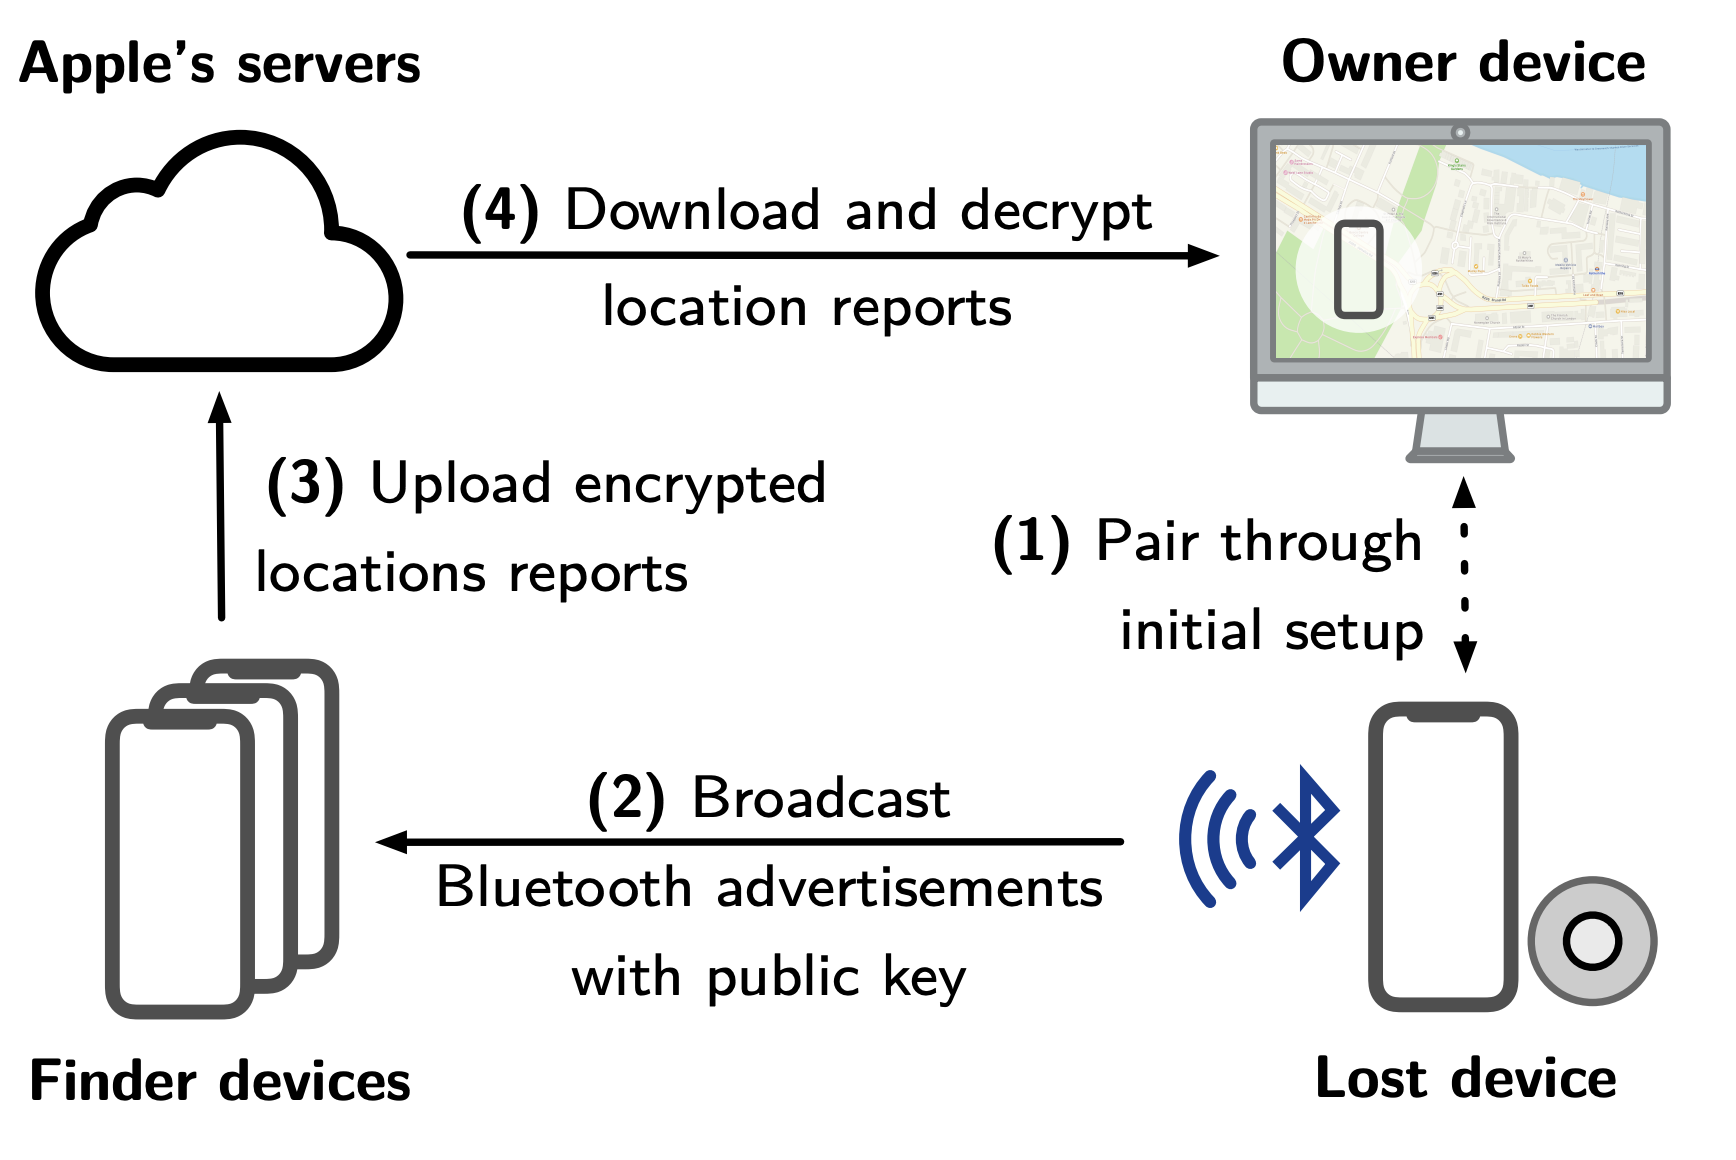
\includegraphics[width=.5\textwidth]{images/process.png}
	\caption{FindMy workflow (image from \cite{whocanfind}).}
	\label{process}
\end{figure}
All Finders scan for FindMy beacons (if the option is enabled in Settings).
This kind of devices create and upload an encrypted position report to Apple's servers whenever they receives a beacon in the FindMy advertising format; they are likely to use less energy and bandwidth because they gather reports over time and transfer them in batches on a regular basis. The evaluation done in \cite{whocanfind} discovered that ``the median time from generating to uploading a location report is 26 minutes and the delay can increase to several hours if the finder device is in low power mode".

\subsubsection{Cryptography} \label{sec:crypto}
We will now delve more into the Cryptography protocols used. 
\paragraph{Advertisement keys}\label{keys}
FindMy utilizes Elliptic Curves \cite{ec}; according to \cite{aps,whocanfind}, ``the process to generate \textit{advertisement keys} is the following:
\begin{enumerate}
  \item Each owner device generates a private/public key pair
  $(d_0, p_0)$ on the NIST $P-224$ curve and a $32$-byte symmetric key $SK_0$ that together form the master beacon key. Those keys are never sent out via BLE and are used to derive the rolling advertisement keys included in the BLE advertisements. Note that device tracking is hard since rolling keys can be deterministically derived if and only if one knows the initial input keys $(d_0, p_0)$ and $SK0$.
  \item Advertisement keys $(d_i,p_i)$ are iteratively calculated as follows using the ANSI X.963 key derivation function $KDF$ \cite{ANSI} with $SHA-256$ \cite{sha} and a generator $G$ of the NIST P-224 curve:
  \begin{align}
    SK_i &= KDF(SK_{i-1},\ 'update',\ 32) \\
    (u_i, v_i) &= KDF(SK_i,\ 'diversify',\ 72) \\
    d_i &= (d_0 * u_i) + v_i \\
    p_i &= d_i * G
  \end{align}
  where Equation $(1)$ derives a new symmetric key from the last used symmetric key with 32 bytes length. Equation $(2)$ derives the so-called “anti-tracking” keys $u_i$ and $v_i$ from the new symmetric key with a length of $36$ bytes each. Finally, Eqs. $(3)$ and $(4)$ create the advertisement key pair via EC point multiplication using the anti-tracking keys and the master beacon key $d_0$".
\end{enumerate}

\paragraph{Key synchronization}
To download and decode location information, the advertisement keys must be accessed by all owner devices. In order to synchronize the master beacon keys, FindMy uses iCloud to encrypt a property list file in the Galois/Counter mode of the Advanced Encryption Standard (AES-GCM) \cite{gcm}. The file's decryption key is kept in the iCloud keychain underneath the label “Beacon Store”.

\paragraph{Encryption}
Each BLE beacon contains an Elliptic Curve public key $p_i$. When a finder device intercepts a beacon, it saves its location and encrypts it using the $p_i$ key; Subsequently, it uploads the packet to Apple's servers.
OF uses the Elliptic Curve Integrated Encryption Scheme (ECIES), which generates a shared secret that is utilized to encrypt the report through an ephemeral key exchange (Elliptic Curve Diffie-Hellmann (ECDH)). According to \cite{whocanfind}, ``the finder’s encryption algorithm works as follows:
\begin{enumerate}
  \item Generate a new ephemeral key $(d', p')$ on the NIST P-224 curve for a received FindMy lost advertisement.
  \item Perform ECDH using the ephemeral private key $d'$ and the advertised public key $p_i$ to generate a shared secret.
  \item Derive a symmetric key with ANSI X.963 $KDF$ on the shared secret with the advertised public key as entropy and SHA-256 as the hash function.
  \item Use the first 16 bytes as the encryption key $e'$.
  \item Use the last 16 bytes as an initialization vector $IV$.
  \item Encrypt the location report under $e'$ and the $IV$ with AES-GCM. 
\end{enumerate} 
The ephemeral public key $p'$ and the authentication tag of AES-GCM are part of the uploaded message". 
All reports are uniquely identified by the SHA-256 hash of $p_i$, which serves as their $ID$, as we can see in Figure \ref{comparison}.

\paragraph{Decryption}
For decryption, the procedure implemented is the reverse of the encryption process. From \cite{whocanfind}, ``An owner device that downloads encrypted location reports follows the inverse of the encryption procedure:
\begin{enumerate}
  \item The owner device selects the proper advertisement keys $(d_i, p_i)$ based on the hashed $p_i$ of the location report.
  \item It performs the ECDH key exchange with the finder’s ephemeral public key $p'$ and the lost device’s private key $d_i$ to compute the symmetric key $e'$ and the $IV$.
  \item Now, the owner can use $e'$ and $IV$ to decrypt the location report."
\end{enumerate}

\begin{figure}
	\centering
	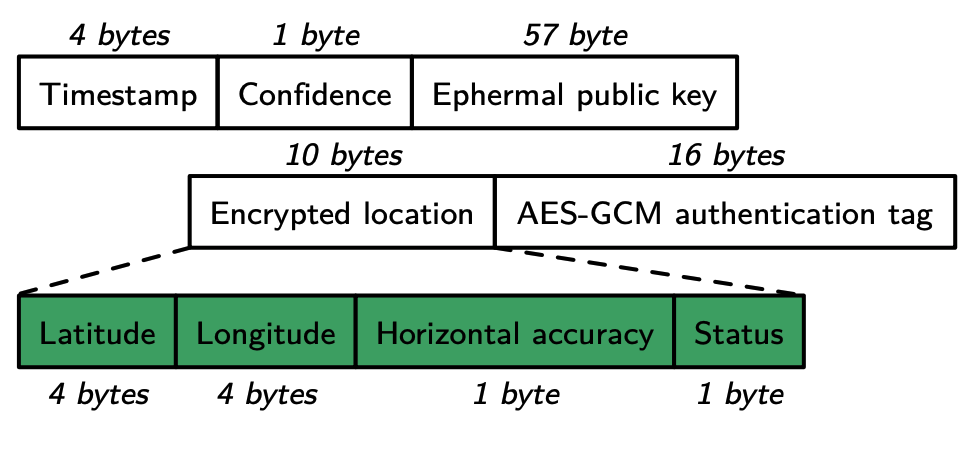
\includegraphics[width=0.5\textwidth]{images/packet.png}\hfill 
	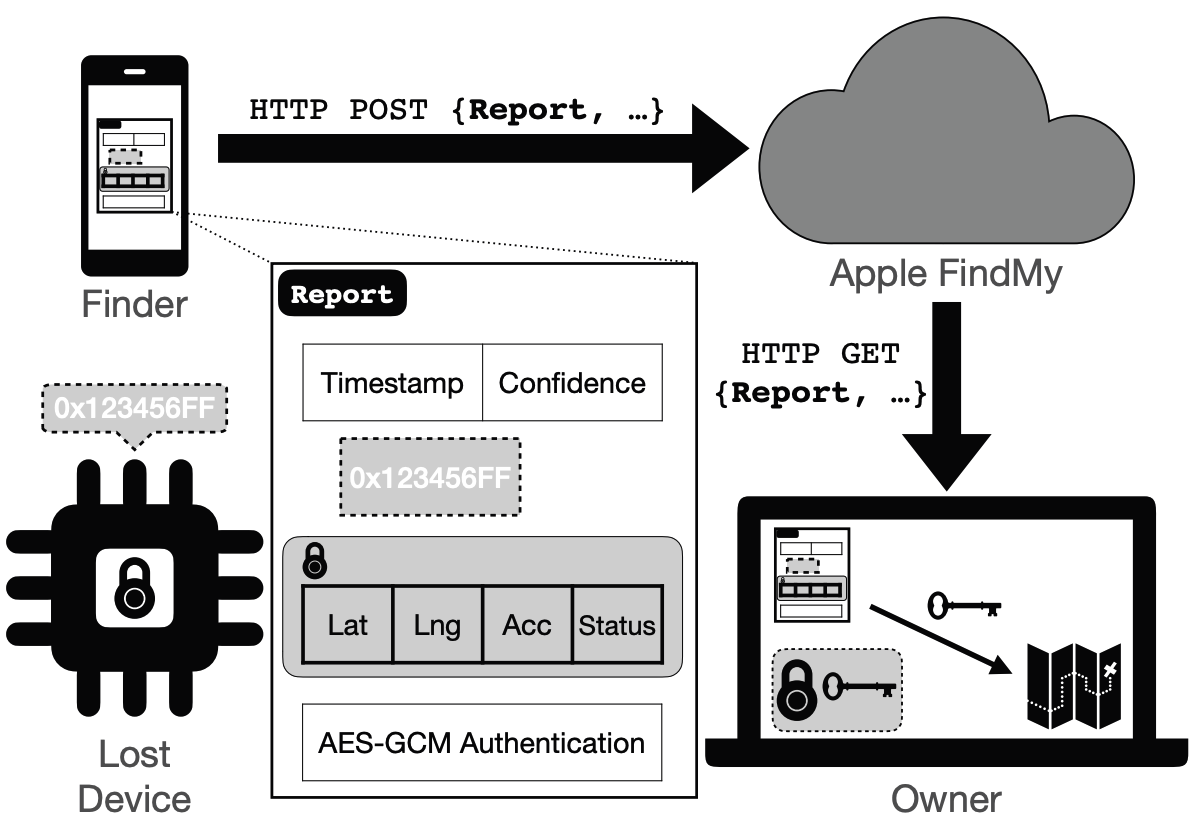
\includegraphics[width=0.5\textwidth]{images/findmysec.png}
	\caption{(a) Binary format of a location report \quad (b) Example of sent payload (images from \cite{whocanfind},\cite{airguard}).}
	\label{comparison}
\end{figure}

\section{Useful applications}\label{appl}
Some useful applications can be the following:
\begin{itemize}
  \item \textit{Travel}: AirTags can be beneficial for travelers. They can attach AirTags to their luggage, making it easier to identify and track their bags during travel. As example, 
  imagine you have just landed from a trip and are eager to grab your bags, waiting endlessly at the carousel can be frustrating. You start worrying that your luggage got lost, but if you've got AirTags inside, you can quickly check if it's still at the airport or somewhere else. Even if it's taking longer than expected, you can keep tabs on it until the airline sorts things out and gets it back to you.
  \item \textit{Pet Tracking}: while not explicitly designed for pets, some users have found AirTags useful for tracking their pets. By attaching an AirTag to a pet's collar, owners can monitor their pet's location and quickly locate them if they wander off. Some tests were conducted in \cite{KittyCatGO2024} and, as we could expect, it seems that the AirTag doesn’t work quite well when in motion, for example, on a moving cat. In \cite{Src2024}, they conducted a test trying to track a dog. As before, the experiment was delusional; they tried to simulate the dog using a plastic box that contained the AirTag and was dropped near a spot where dog walkers regularly walk past it every day. ``Several hours passed before the user received the initial location fix for the lost AirTag. However, this fix was a singular occurrence, and there was no subsequent update for several more hours".
  \item \textit{Child Safety}: similarly to pets, AirTags can give an extra degree of protection for monitoring kids in busy or strange places. Parents can hide or attach an AirTag to their child's clothing or belongings to track their real-time location and ensure there are no dangerous situations where the child gets lost or kidnapped. From \cite{Kelly_2023}: ``ethical debates can arise regarding this issue, as experts have long been worried about the impact of more restrictive parenting on children’s mental health and development". We will not go any deeper on this question since it is a technical report.
  \item \textit{Vehicle Tracking}: AirTags can also be used to track vehicles, such as bicycles, motorcycles or cars, in the same way as the two above. An experiment was done in \cite{Maric2023}, ``an Apple AirTag, a Samsung SmartTag+, and a GPS unit with 3G and 4G compatibility were used to evaluate their performance and determine the most cost-effective solution to track a device; additionally, as a backup measure to these external devices, they used the ConnectedDrive feature on a BMW 3 Series to compare its effectiveness against the other options". Table \ref{vehicles} compares the cost of the used options, data is taken from \cite{Maric2023}. The testing route consists of a 45 km drive and includes four checkpoints. There is no LTE or cell service in close proximity of the last checkpoint; after going back to the starting point, the test ends by evaluating how well each gadget finds the parked automobile once it is in range and idly. The results were as assumed: both aftermarket and built-in GPS units were expected to function properly, transmitting accurate locations via cellular networks, facilitating easy vehicle tracking; however, their main drawback is their cost and the need for ongoing battery monitoring or charging to ensure continuous functionality. In terms of UWB, the AirTag has proven to be a cost-effective solution for vehicle tracking, although it does not have the same update frequency as GPS devices. Interestingly, it was found that the SmartTag+ has a higher update frequency compared to the AirTag.
  \begin{table}[h] 
    \caption{Solutions cost comparison.}
      \centering
      \begin{tabular}{|c|c|c}
        \cline{1-2}
        \textbf{Device}           & \textbf{Cost (\$AUD)}  &  \\ \cline{1-2}
        Apple AirTag              & \$45                   &  \\ \cline{1-2}
        Samsung SmartTag+         & \$60                   &  \\ \cline{1-2}
        GPS tracker with SIM card & \$147 + \$7 per month &  \\ \cline{1-2}
        BMW ConnectedDrive        & From \$119 per year    &  \\ \cline{1-2}
        \end{tabular}
        \label{vehicles}
      \end{table}

  \item \textit{People with Dementia Tracking}: Alzheimer's patients and those suffering from other types of dementia may notice a reduction in their memory for recognizing where they are, which can result in wandering and feelings of being lost or confused. AirTags can offer comfort in these situations and assist caretakers in making sure the person's whereabouts are known; some bracelets have been developed to facilitate the use of Airtags in this context. As we can see in Figure, the Unremovable Bracelet is used to track every movement and it takes two hands to open it, thus making it impossible for your loved ones to take it off.
  \begin{figure}[]
    \centering
    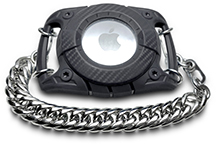
\includegraphics[width=0.35\textwidth]{images/AirT-Blk-Sm.jpg}
    \caption{Unremovable bracelet (image from \cite{bracelets}).}
    \label{img:controller}
  \end{figure}
  \item \textit{Intrusion detector}: an innovative usage can be as an intrusion detector. Imagine a scenario where you want to check whether anyone is near your remote cabin; if you place an AirTag hidden somewhere near it, if someone with an iPhone passes nearby, then you will be noticed in minutes, since the intruder's device will forward to iCloud the AirTag position.
  \item \textit{Wallet tracker}: this can be the most obvious application of this kind of device. A lot of wallets with built-in space for the AirTag were created, making it easier for the user to track their wallets.
  \item \textit{Supermarket shelf localizer}: an interesting usage can be to act as a localizer inside a supermarket. Imagine a scenario where an elderly person goes grocery shopping in a very large supermarket and gets lost inside. In such cases, an application could be developed using Apple's APIs to help locate all the shelves for the user, utilizing the precision finding offered by UWB. In the future, integrated tablets could be available on shopping carts, allowing users to locate shelves using navigation (Precision Finding) provided in FindMy.
\end{itemize}

\subsection{Mods}
After some Internet research, the author discovered that the AirTag has been modified in certain ways. For instance, in \cite{telecomando} A. Catley has attached the AirTag to a remote controller and is powering the AirTag components using the host's battery. This could be very useful in situations in which the remote controller gets lost in the house; thanks to Precision Finding, the owner can find it easily. Figure \ref{img:controller} shows the final result.
Now, imagination knows no bounds, and there are always innovative ways to utilize AirTags.
\begin{figure}[]
	\centering
	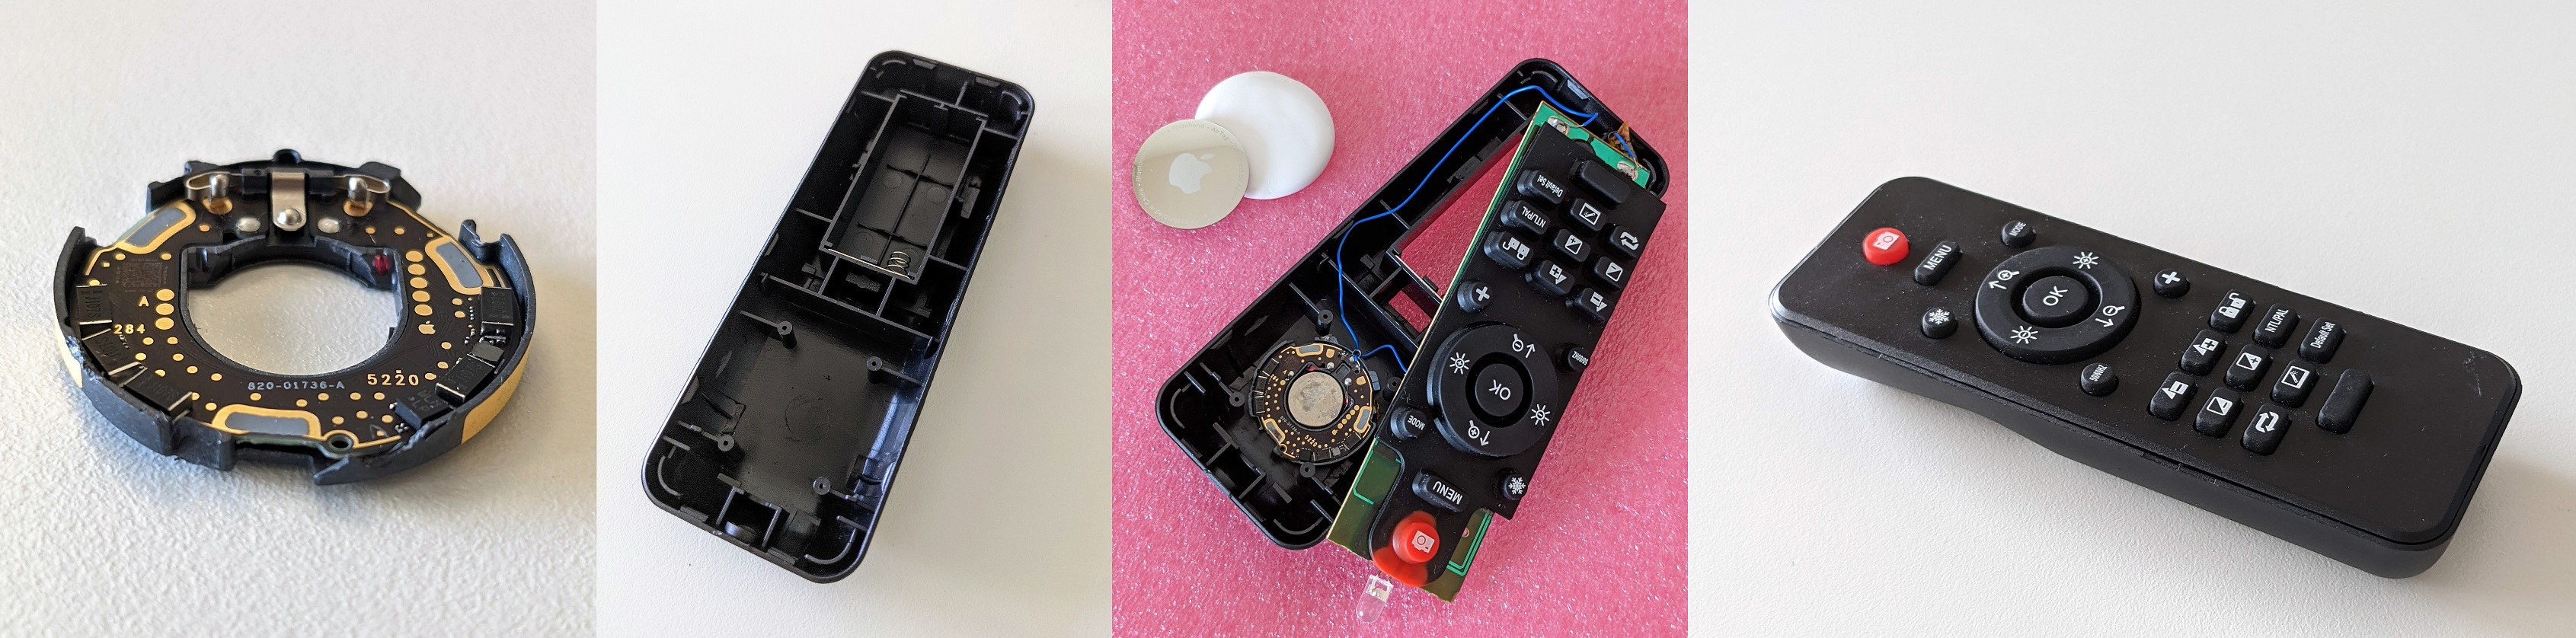
\includegraphics[width=\textwidth]{images/remote.jpg}
	\caption{AirTag inside a remote control (images from \cite{reverse}).}
	\label{img:controller}
\end{figure}


\section{Conclusion}
In conclusion, the paper provided a comprehensive exploration of various technological aspects. The AirTag technology and FindMy architecture offer a smart solution to address the tracking issue by intelligently utilizing the network of Apple devices worldwide, all at a much lower price compared to competitors.Other technologies also utilize the same principle, but AirTag's strength lies in the Apple device network present worldwide. Currently, according to \cite{Lin}, Apple holds $29.27\%$ of the smartphone market share. This explains why the service performs so well. There are numerous possibilities for the future, some of which have been discussed in Section \ref{appl}. One potential future development of this technology could involve integrating it into everyday tools to add precision tracking capabilities. For instance, integrating FindMy into shopping carts in supermarkets to locate shelves. In the future, this technology can only improve as the network of Apple devices supporting both FindMy and Precision Finding continues to grow with the purchase of new iPhones (which now integrate the UWB chip). Security-wise, vulnerabilities highlighted in Section \ref{sec:vuln} need to be addressed, as user privacy is paramount, and a company like Apple cannot afford to ignore the issue.
\printbibliography
\nocite{*}

\end{document}